\documentclass[12pt,a4paper]{article}

\usepackage[T1]{fontenc}
\usepackage[utf8]{inputenc}
\usepackage[margin=2.5cm]{geometry}
\usepackage{graphicx}
\usepackage[hidelinks]{hyperref}
\usepackage{fancyhdr}
\usepackage{lastpage}
\usepackage{appendix}
\usepackage{color}
\usepackage{palatino}
\usepackage{changepage}
\usepackage{subcaption}
\usepackage{enumitem}
\usepackage{csquotes}
\usepackage{verbatim}
\usepackage{minted}
\usepackage[ruled,vlined]{algorithm2e}

\usemintedstyle{default}
\setminted{
  linenos=true,
  breaklines=true,
  fontsize=\small,
  frame=single,
}

\title{Binary Space Partitions}
\author{Carlos Requena López}

%% Fancy layout
\pagestyle{fancy}
\lhead{Binary space partitions}
\chead{}
\rhead{}
\lfoot{}
\cfoot{}
\rfoot{Page \thepage\ of \pageref{LastPage}}
\renewcommand{\headrulewidth}{0.4pt}
\renewcommand{\footrulewidth}{0.4pt}


%%% --- %%% --- DOCUMENT START --- %%% --- %%%
\begin{document}
\maketitle
\thispagestyle{empty}
\tableofcontents
\newpage
%%% Counting pages now %%%
\pagestyle{fancy}
\setcounter{page}{1}


\section{Introduction}

This first assignment deals with recursive autopartitioning of a two
dimensional space into a binary tree. Autopartitions, in contrast to
partitions, are performed extending the supporting lines of the
segments already present on the plane.

In particular, with partitions, we stop executing the algorithm when
there is one segment or object per partition. The autopartition stops
when no more segments can be extended.

Having direct application in computer graphics, the most interesting
parameter when considering these partitions in the size of the
generated tree, since that's what is used in practice to decide what
to render first in the scene of a computer screen.

\section{Analysis and expectations}

We define the algorithm RandAutopart in algorithm \ref{algo}, where we
can see that the tree grows every time a line segment intersects
another segment. The intersected segment is essentially split in two
and given to the left and right children of that node.

\begin{algorithm}[h]
  \SetAlgoLined
  \KwIn{A set S of segments}
  \KwOut{The autopartition binary tree}

  \nl Pick a random permutation of S and take the first element\;
  \nl Extend this element into a line and create a node with it in the tree\;
  \nl Filter the segments strictly to the left in the \texttt{left}
  child\;
  \nl Filter the segments strictly to the right in the \texttt{right}
  child\;
  \nl \For{segment in all segments that intersect}{
    \nl add its subsegment laying on the left part to the
    \texttt{left} child\;
    \nl add its subsegment laying on the right part to the
    \texttt{right} child\;
  }
  \nl \While{\texttt{left} or \texttt{right} have segments in them}{
    \nl Repeat this procedure recursively on both sets\;
  }
\caption{\bf RandAutopart}
\label{algo}
\end{algorithm}

We are interested in making this tree as small as possible, to make it
efficient for other applications (the painter's algorithm, for
example) to traverse the tree and render the scene as fast as
possible. The upper bound on the size of the tree we consider is given
in Eq. \ref{eq:upper-bound}.

\begin{equation}
  \label{eq:upper-bound}
  n + 2 \sum_u \sum_{i=1}^{n-1} \frac{1}{i+1} \leq n + 2nH_n
\end{equation}

This upper bound found in the literature, specifically in
\cite[p.~14]{Motwani:1995:RA:211390}, corresponds to the upper bound of the
random algorithm for any input. The expectation would be for this
boundary to be closer when choosing the worst possible input (segment
positioning wise) and further away when adding randomness to the input
and even more when giving the most trivial input possible: parallel
segments, in which case the number of partitions would be $n+1$.

The algorithm will be therefore tested with random inputs of different
characteristics too try and see what makes a bad or a good input, in
order to get closer to this upper bound without ever exceeding it.

\section[Implementation]{Implementation\footnote{Code can be found at
    \url{https://github.com/carlosgeos/bspace-part}}\footnote{An
    executable \texttt{.jar} file can be downloaded from
    \url{https://github.com/carlosgeos/bspace-part/releases}}}

$n$ disjoint segments are generated and placed on a $H\times W$
canvas, where $H$ is the height and $W$ the width, both in pixels.

The first element of a random permutation of those $N$ segments is
taken, its supporting line extended, and the host space (the plane)
partitioned in two. The same procedure is applied recursively to

In order to know which segments another line intersects, some
primitive geometry operations have to be implemented. Since this is
done from scratch however, we expect them to not be as robust as the
ones some external library could provide. These operations include:

\begin{itemize}
\item Testing to which side a point is with respect to a line segment
  (of if it is on the line).
\item Testing whether a segment is on one side or the other of a
  segment (or if it is colinear).
\item Testing whether a segment could potentially intersect another if
  its supporting line is extended.
\item Testing whether two segments intersect each other.
\item Determining the coordinates of the intersection of a line and a
  segment.
\end{itemize}

Most operations rely on calculating the orientation determinant
between the line segment defined by two points and a third point.

The generated segments' coordinates are integers to begin with and
Clojure uses a \texttt{Ratio} type to make arithmetic calculations as
exact as possible and to avoid floating point rounding errors. This
comes at the expense of performance, which is not an issue.

In addition, this implementation tries to handle degenerate and
special cases as much as possible (colinear segments,
segment-on-segment, vertical segments, out-of-bounds segments, segment
of size 0 - points, tangent segments, etc).

For example, for the input shown in figure \ref{fig:sample-input} the
corresponding partition tree is the following (there are no
intersections in this case):

\begin{minted}[label=sample-output]{clojure}
"BSpace partitions"
{:seg {:a {:x 492, :y 556}, :b {:x 388, :y 932}},
 :left
 {:seg {:a {:x 625, :y 409}, :b {:x 530, :y 745}},
  :left (),
  :right
  {:seg {:a {:x 626, :y 355}, :b {:x 588, :y 243}},
   :left (),
   :right ()}},
 :right
 {:seg {:a {:x 264, :y 626}, :b {:x -8, :y 571}},
  :left (),
  :right
  {:seg {:a {:x 88, :y 291}, :b {:x 36, :y 79}},
   :left (),
   :right ()}}}
\end{minted}

\begin{figure}[ht!]
  \centering
  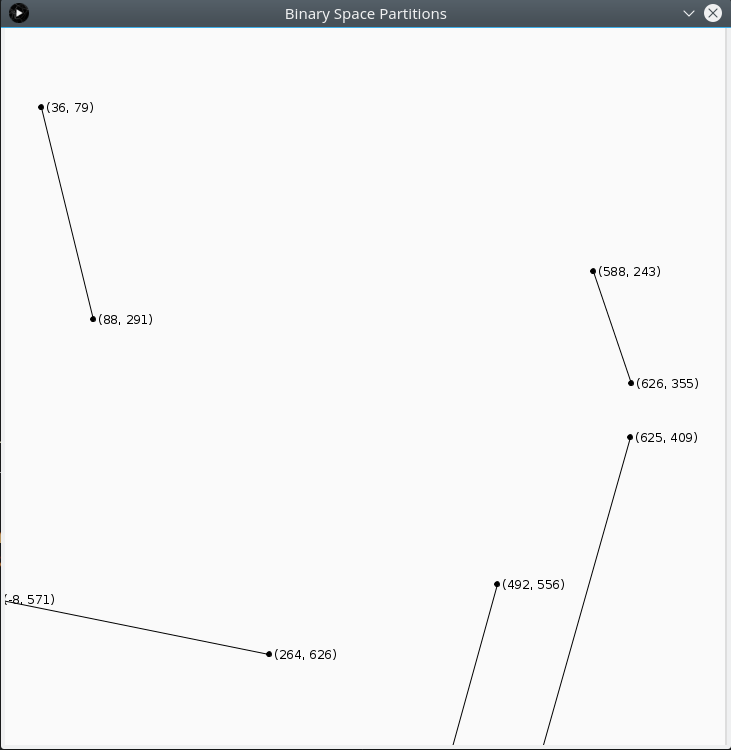
\includegraphics[width=0.7\textwidth]{img/sample-input.png}
  \caption{Five random segments on a 720x720 canvas}
  \label{fig:sample-input}
\end{figure}

From the resulting tree, we can count the number of original and newly
generated segments. The same result could be obtained counting these
during the execution of the main algorithm, to avoid walking the tree
once afterwards.

\section{Results}

Table \ref{tab:results} shows a summary of the simulations performed
on random inputs. Overall, we can see that the size of the tree is
quite distant from the upper bound.

\begin{table}[ht!]
  \centering
  \begin{tabular}[center]{||c|c|c|c|c||}
    \hline
    \# of segments & Canvas size (px) & Max segment size (px) & Tree size
    & Upper bound \\
    \hline \hline
    10 & 720x720 & 50 & 12 & 68 \\
    10 & 720x720 & 50 & 11 & 68 \\
    10 & 720x720 & 250 & 14 & 68 \\
    100 & 720x720 & 50 & 132 & 1137 \\
    100 & 720x720 & 50 & 137 & 1137 \\
    100 & 720x720 & 250 & 221 & 1137 \\
    1000 & 720x720 & 50 & 2213 & 15970 \\
    1000 & 720x720 & 50 & 2262 & 15970 \\
    1000 & 720x720 & 250 & 2808 & 15970 \\
    2000 & 720x720 & 50 & 5179 & 34713 \\
    2000 & 720x720 & 5 & 2395 & 34713 \\
    2000 & 720x720 & 250 & 6710 & 34713 \\
    5000 & 720x720 & 250 & 16227 & 95945 \\
    10000 & 720x720 & 3 & 12698 & 205752 \\
    \hline
  \end{tabular}
  \caption{Simulation results}
  \label{tab:results}
\end{table}

One can appreciate that making the segment length very small (3 or 5
pixels, such as in fig. \ref{fig:sparse-input} and
fig. \ref{fig:sparse-input2}), makes the difference between the size
of the tree and the upper bound grow. This is due to the extended
lines cutting very few segments in the sparse region.

\begin{figure}[ht!]
  \centering
  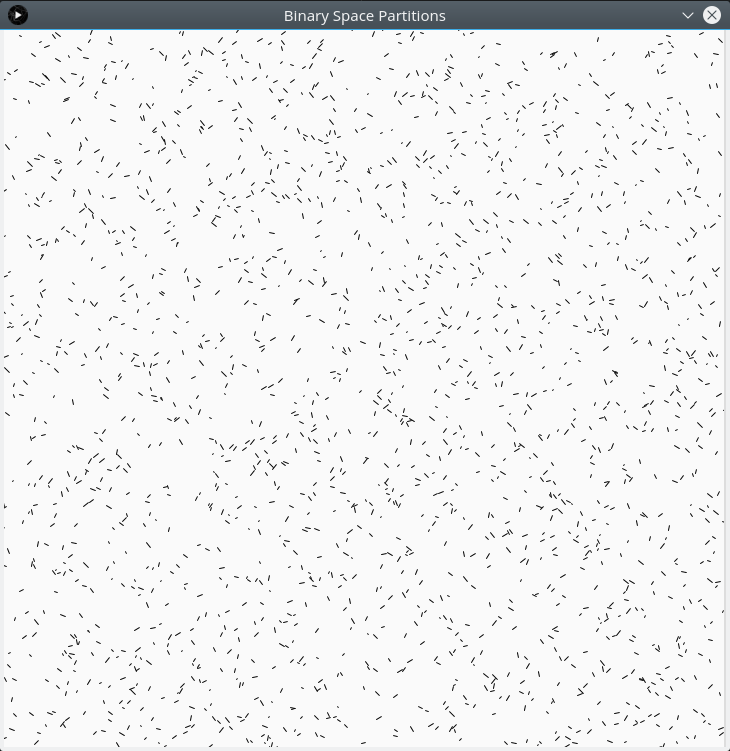
\includegraphics[width=0.7\textwidth]{img/sparse-input.png}
  \caption{Sparse segments. n = 2000}
  \label{fig:sparse-input}
\end{figure}

Another observation is that taking half the segment length affects the
same way the size of the tree as doubling the parameters
\texttt{WIDTH} and \texttt{HEIGHT} of the canvas, which is logical.


\begin{figure}[ht!]
  \centering
  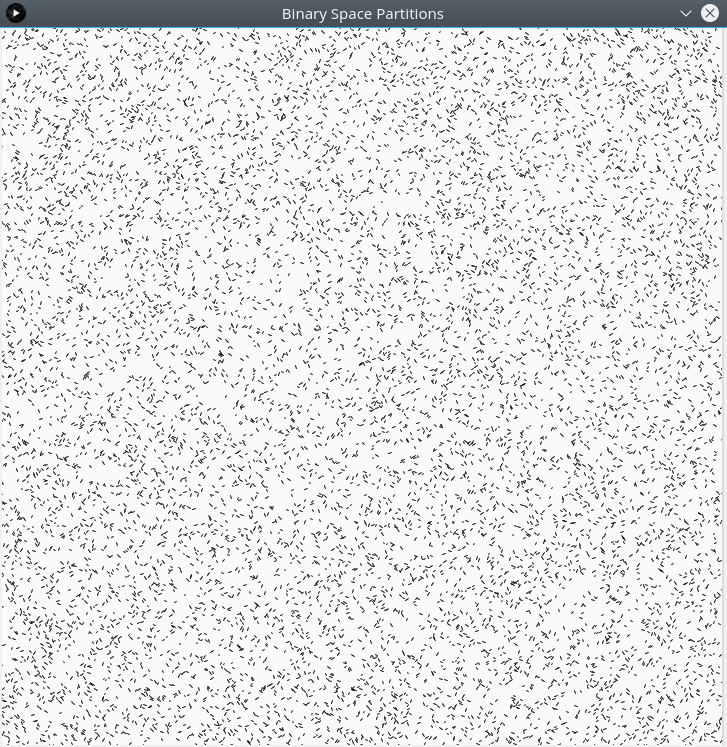
\includegraphics[width=0.7\textwidth]{img/sparse-input10000.png}
  \caption{Sparse segments. n = 10000}
  \label{fig:sparse-input2}
\end{figure}

\begin{figure}[ht!]
  \centering
  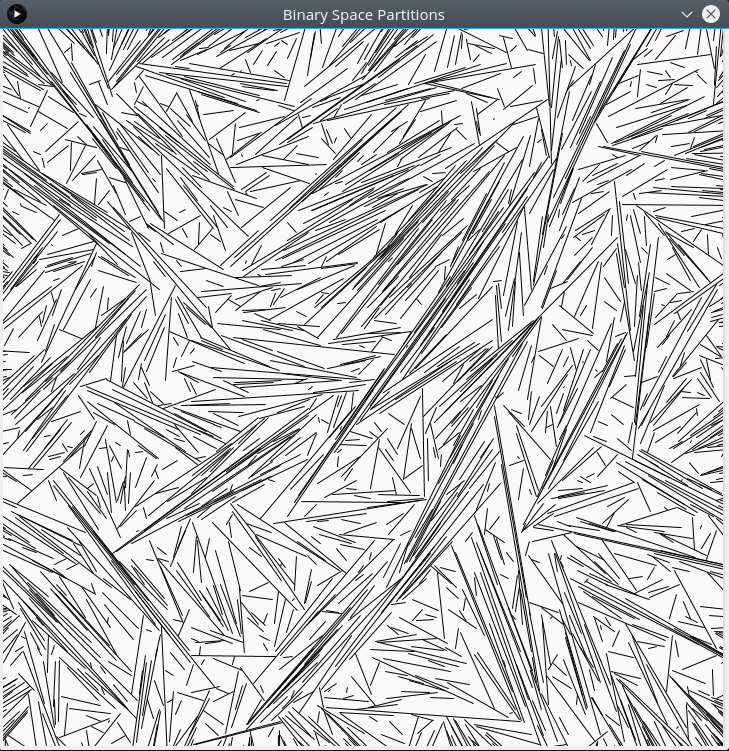
\includegraphics[width=0.7\textwidth]{img/bad-input2000.png}
  \caption{``Bad'' input. n = 2000}
  \label{fig:bad-input}
\end{figure}

One of the worst inputs that could be found is shown in
fig. \ref{fig:bad-input}, although the size of the tree stays well
below the threshold. The approach to design the worst input possible
would be to make the algorithm choose a ``bad'' segment every time. A
``bad'' segment intersects with all or most other segments in its
region, splitting them and generating subsegments, more partitions and
incrementing the tree size. But the strength of the algorithm is
precisely that we do not know which segment is going to pick next,
hence the power of randomisation.

\section{Conclusion}

The simulations stay below the upper bound given in
Eq. \ref{eq:upper-bound}, as expected, and it does so regardless of
what the input is, since that result was obtained with respect to the
randomness of the algorithm and not the structuredness (or lack of it)
of the input.

If we could place the segments in the space in such a way that the
algorithm would have no choice but to pick a bad segment at each
iteration, thereby ``defeating'' the algorithm, we would see the tree
size get closer to the upper bound.

\appendix
\section{Appendix - code listing}

\inputminted[label=common.clj]{clojure}{../src/bspace_part/common.clj}
\inputminted[label=geometry.clj]{clojure}{../src/bspace_part/geometry.clj}
\inputminted[label=core.clj]{clojure}{../src/bspace_part/core.clj}

\nocite{*}
\bibliographystyle{plain}
\bibliography{refs}

\end{document}
